% ---------------------------------------------------------------------------
\subsection*{Estudo de convergência da simulação CFD}
% Critério: convergência de malha + independência da solução, justificar a malha.

%O estudo de independência de malha foi realizado para quatro configurações
%de malha. \tbd{Confirmar o ângulo de ataque.}
%A Tabela~\ref{tab:malhas} resume as malhas testadas e a
%Figura~\ref{fig:independencia_cfd} apresenta os coeficientes aerodinâmicos e
%o indicador de eficiência das malhas.

De forma a garantir que os resultados das simulações com recurso a CFD não são afetadas pela resolução da malha, é importante realizar um estudo de independência da malha. Para o efeito, foram realizadas simulações para quatro malhas diferentes, todas para um ângulo de ataque de 5\textdegree.

Segundo Celik et al.~\cite{mesh_independence}, para um estudo de independência de malha devemos ter uma razão de refinamento, $r = h_\text{coarse} / h_\text{fine}$, superior a 1.3. Foi portanto utilizado $r\approx1.4$.

É de destacar o facto de, para as diferentes malhas, a altura da primeira \textit{inflation layer} manteve-se absoluto, ao invés de relativo ao tamanho da célula, de forma a assegurar um $y^+$ constante ao longo dos diversos tamanhos da célula exterior. Isto provoca, no entanto, diferenças na transição entre a \textit{inflation layer} e o restante domínio. As configurações da geração das \textit{inflation layers} foram determinadas com foco principal na malha com célula exterior com $h=0.10$.

\begin{table}[H]
  \centering
  \caption{Estudo de independência de malha.}
  \label{tab:malhas}
  \begin{tabular}{lccc}
    \toprule
    $h_\text{cel. exterior}$ & N.º de células & $c_l$ & Variação de $c_l$ [\%] \\
    \midrule
    0,14 & \tbd{} & \tbd{} & --- \\
    0,10 & \tbd{} & \tbd{} & \tbd{} \\
    0,07 & \tbd{} & \tbd{} & \tbd{} \\
    0,05 & \tbd{} & \tbd{} & \tbd{} \\
    \bottomrule
  \end{tabular}
\end{table}

\begin{figure}[H]
  \centering
  \begin{subfigure}[c]{0.48\linewidth}
    \centering
    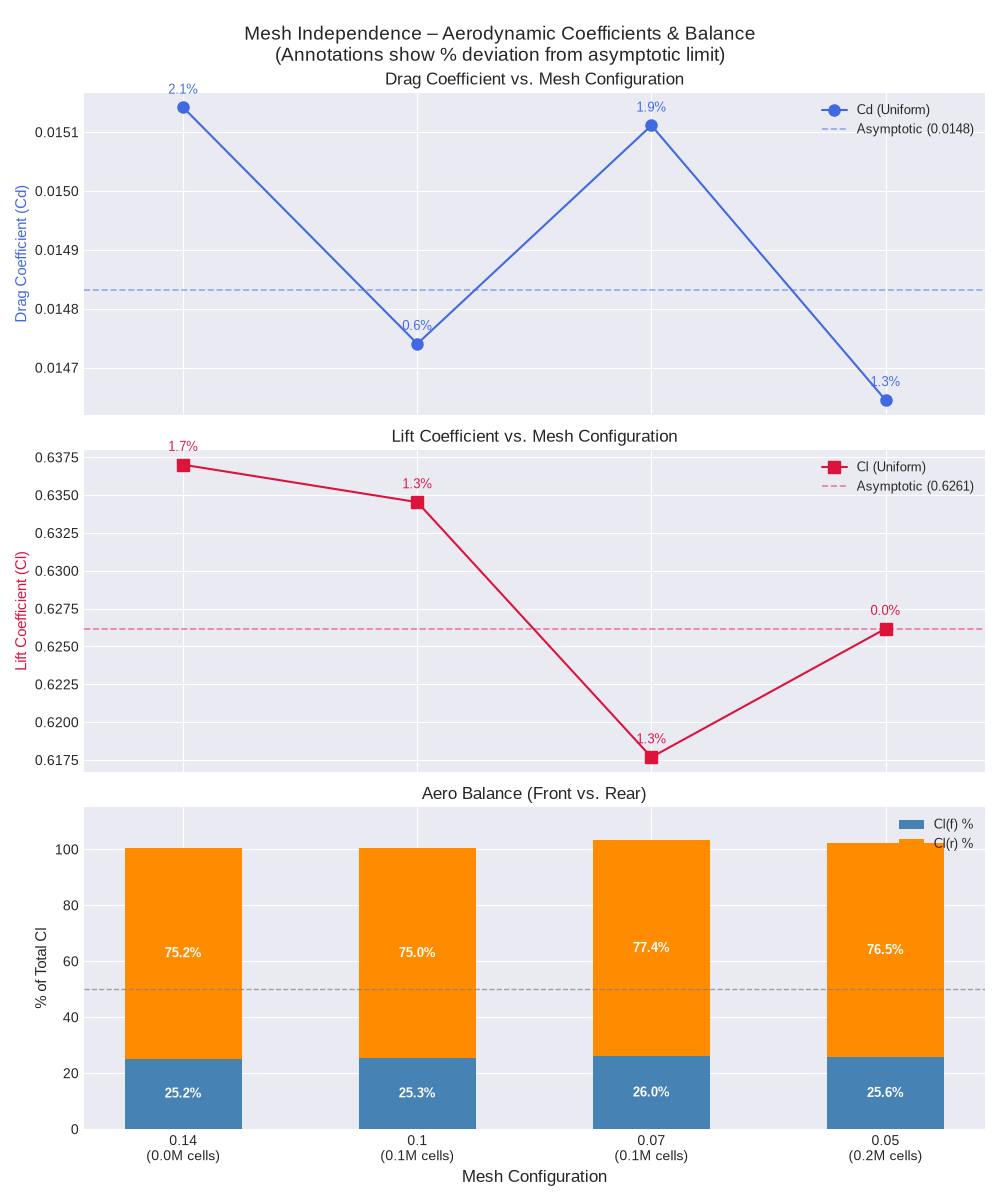
\includegraphics[width=\linewidth]{../CFD/graficos-mesh-independence/Figure_1.png}
    \caption{Coeficientes aerodinâmicos e equilíbrio aerodinâmico.}
  \end{subfigure}\hfill
  \begin{subfigure}[c]{0.48\linewidth}
    \centering
    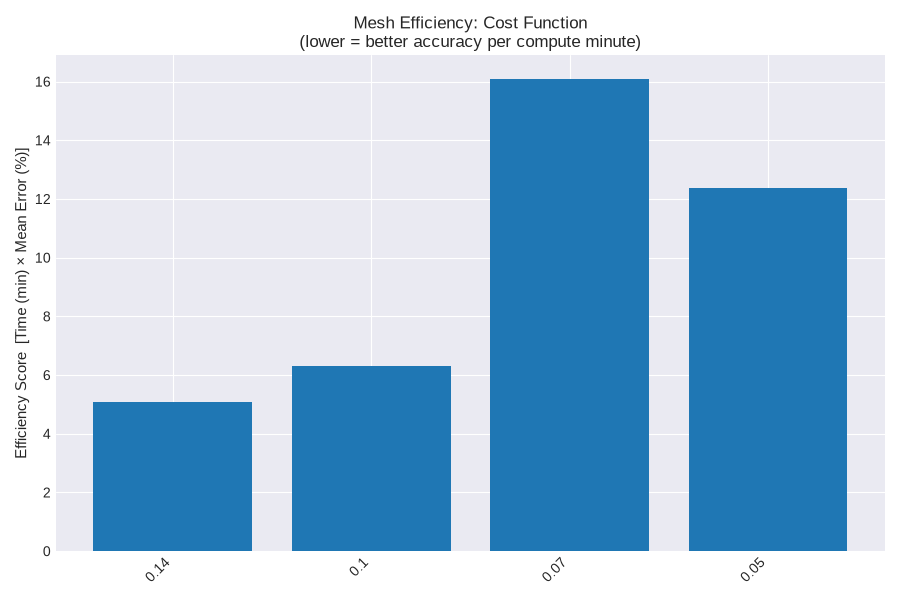
\includegraphics[width=\linewidth]{../CFD/graficos-mesh-independence/Figure_5.png}
    \caption{Indicador de eficiência computacional.}
  \end{subfigure}
  \caption{Estudo de independência da solução CFD e eficiência das malhas.}
  \label{fig:independencia_cfd}
\end{figure}

A Figura~\ref{fig:custo_yplus_cfd} apresenta os tempos de geração da malha
e de simulação, bem como os valores médio, mínimo e máximo de $y^+$ para cada
configuração de malha.

\begin{figure}[H]
  \centering
  \begin{subfigure}[c]{0.48\linewidth}
    \centering
    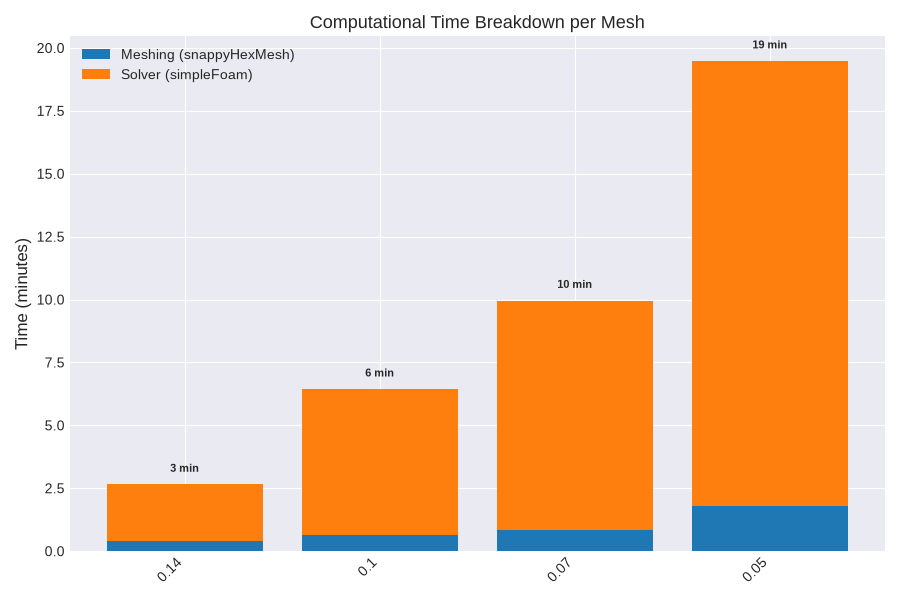
\includegraphics[width=\linewidth]{../CFD/graficos-mesh-independence/Figure_2.png}
    \caption{Tempos de geração de malha e simulação.}
  \end{subfigure}\hfill
  \begin{subfigure}[c]{0.48\linewidth}
    \centering
    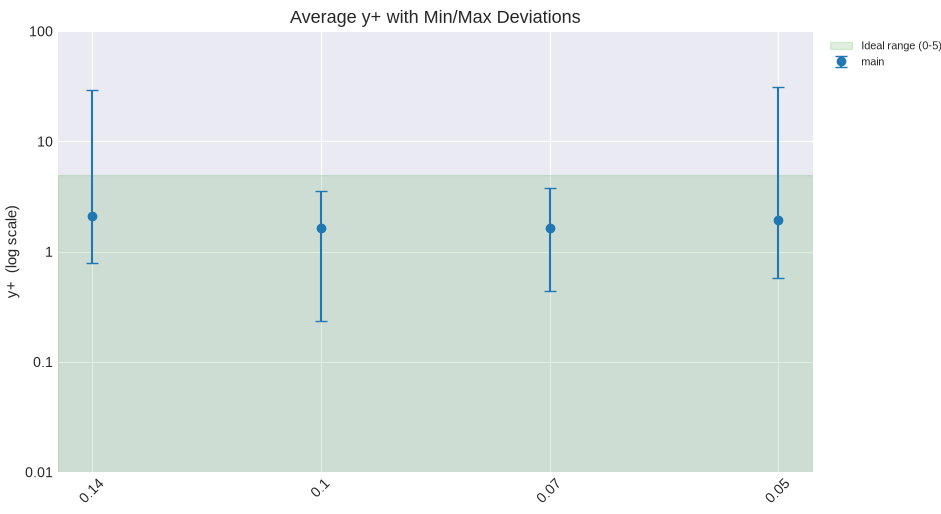
\includegraphics[width=\linewidth]{../CFD/graficos-mesh-independence/Figure_3.png}
    \caption{Estatísticas de $y^+$ por malha.}
  \end{subfigure}
  \caption{Custo computacional e indicadores de resolução junto à parede.}
  \label{fig:custo_yplus_cfd}
\end{figure}

\tbd{Análise (sem IA): explicar os resultados do estudo de independência,
identificar o parâmetro de refinamento e justificar a malha escolhida,
considerando a precisão, o tempo de cálculo e a resolução da camada limite.}

\tbd{A figura \texttt{CFD/graficos-mesh-independence/Figure\_4.png},
relativa aos indicadores de qualidade da malha, não foi inserida para
poupar espaço. Avaliar se é necessário incluí-la.}

